%%% Local Variables:
%%% mode: latex
%%% TeX-master: "../report"
%%% End:

\subsubsection{motivation}
We wanted to explore the concept of private and
confidential communication as we feel that commonly used messaging
solutions do not provide enough. We aim to do so using RSA as our
encryption standard and using TLS for our authentication.
...
...
...


scenario
create a scenario or just more motivation??
discuss:

\subsubsection{security analysis}
There are many ways to attack a system depending on what you want and
what your attacking. We aim to have confidentiality and privacy by
securing our `application'~\todo{get better word} from at least the
following attacks:
\begin{itemize}
\item Man in the middle(MtiM)
\item Chosen-ciphertext attack (CCA)
\item Ciphertext-only attack (COA)
\item Time/memory tradeoff attacks (TMTA)
\end{itemize}

\paragraph{Confidentiality} is protecting information from disclosure
to unauthorized parties. Information is a currency bank accounts,
credit card numbers, social security trade secrets, all this data can
be used maliciously therefore it needs to be protected. A key element
of keeping our data confidental is encryption. Encryption esures that
only the people with the key can access the data. Again there are
several ways to break encryption such as CCA, COA, TMTA or simply
obtaining the private key of the target. To secure yourself from most
of these attacks the encrypton key should at least be above 128 bits,
as a smaller key has been shown to be breakable. In our case we use
the asymetric encryption RSA with 256 bit public and private keys.

\paragraph{Privacy} Is a concern for many people
\paragraph{Anonymity}
is a cornerstone of the internet, most comments are done
anonymously using unidentifiable pseudonyms. Though these usernames
can be used to identify the user they have the possibility of being
separated and anonymous from the actor. Anonymity on the internet is
basically that a comment you state will not be able to be tracked back
to you.

A big problem for anonymity is IP adresses as they serve as an virtual
address. These can be mapped to your Internet Service Provider (ISP),
who can provide customer information as they know what IP addresses
are leased to whom. This does not implicate a specific indivudual but
provides regional information and is powerful circumstantial
evidence.\todo{good bad sides of anon?}

\paragraph{Authentication}of information is important because of
vulnerabilities ot a malicious party either pretending to be you or
someone you know. Without authentication the malicious party (Eve) can
sit in between Bob and Alices conversation and pretend to be either of
them. This is where authentication plays an important role. With
authenticfication we ensure identity of the person we are speaking
with. This is can be done several different ways but in our case we
decided to use Transport Layer Security (TLS) which predecessor is,
Secure Sockets Layer (SSL).

%% \begin{wrapfigure}{r}{0.4\textwidth}
%%   \vspace{-10pt}
%%   \begin{center}
%%     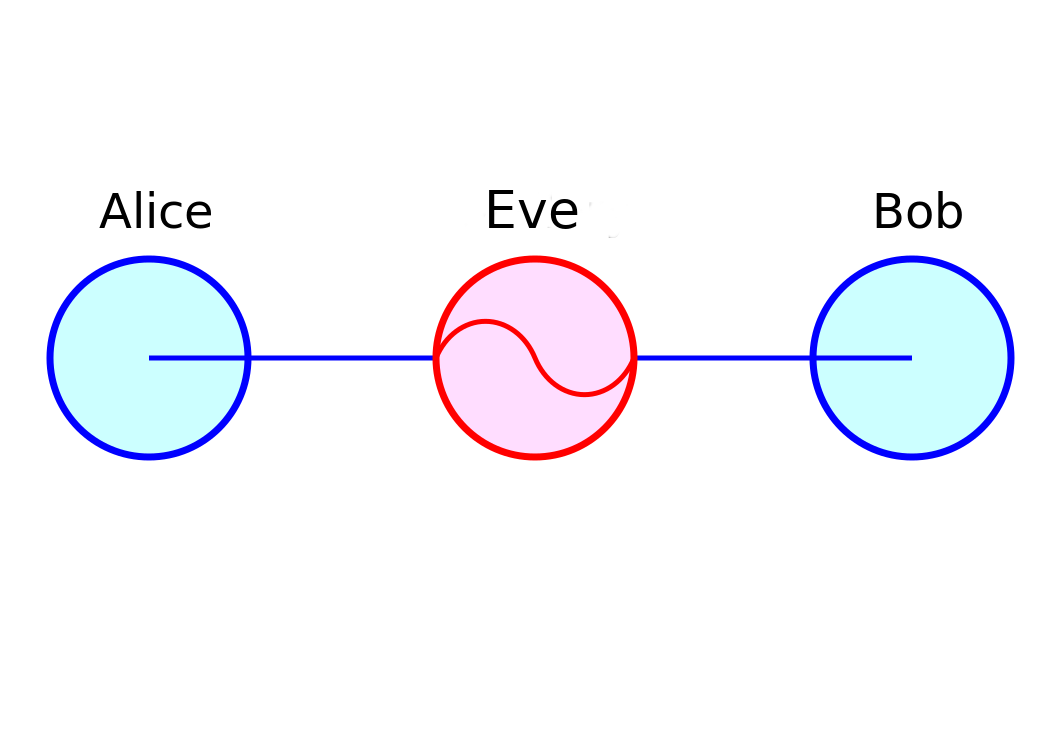
\includegraphics[width=0.3\textwidth]{figures/mitm}
%%   \end{center}
%%   \vspace{0pt}
%%   \caption{\label{fig:demographic} Target demographic}
%%   \vspace{-10pt}
%% \end{wrapfigure}
